\section{Gleichstromumrichter}
\subsection{Buck-Converter (Tiefsetzsteller)}
Ein einfacher Tiefsetzsteller könnte auch mit einem Spannungsteiler bebaut werden.
Die Verlustleistung würde jedoch $P_{V} = R_{1} \cdot I_{1}^2$ betragen.


Grundgleichungen:\\
$V_{1}= i_{L} \cdot R + L\dfrac{di_{L}}{dt}, t \in [0; T_{e}]$\\
$0 = i_{L} \cdot R + L\dfrac{di_{L}}{dt}, t \in [T_{e}; T_{s}]$ ($L\dfrac{di_{L}}{dt}$ ist dabei die Spannung, welche die Induktivität abgibt
$\rightarrow$ Quelle in diesem Fall)\\\\

\begin{minipage}{ 0.5 \linewidth}
  Durch das Lösen der Grundgleichungen erhält man die den Verlauf des Stromes:\\\\
  
  $i_{L} = \frac{V_{1}}{R_{1}}+\frac{V_{1}}{R_{1}} \cdot \frac{-1+e^{\frac{-T_{a}}{\tau}}}{1-e^{\frac{-T_{s}}{\tau}}} \cdot e^{\frac{-t}{\tau}}, t \in [0; T_{e}]$\\\\
  $i_{L} = \frac{V_{1}}{R_{1}} \cdot \frac{1-e^{\frac{-T_{e}}{\tau}}}{1-e^{\frac{-T_{s}}{\tau}}} \cdot e^{\frac{-(t+T_{e})}{\tau}}, t \in [T_{e}; T_{s}]$ mit $\tau = \frac{L_{1}}{R_{1}}$\\\\
  und folgende Ein- und Ausschaltzeiten:\\\\
  $T_{a} = -\tau \cdot \ln\frac{i_{Lmin}}{i_{Lmax}}$ mit $\tau = \frac{L_{1}}{R_{1}}$\\\\
  $T_{e} = -\tau \cdot \ln\left(\frac{\zaehlerBuck}{\nennerBuck}\right)$\\\\
  $T_{s} = T_{e} + T_{a}$
\end{minipage}
\hfill
\begin{minipage}{0.5 \linewidth}
  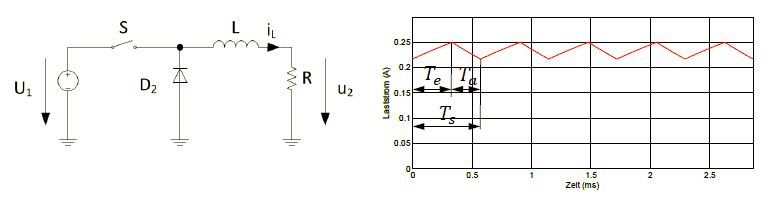
\includegraphics[width = \textwidth]{./pictures/buckConverter}
\end{minipage}
